\chapter{Literature Review}
\label{background}
\section{Machine Learning} \label{background_machinelearning}
When developing a computer algorithm which takes some data as an input and returns an output,
we will usually look at the underlying mechanism as to how we come to that conclusion. However it is not
always possible to know what is the underlying mechanism that produces an output
given certain inputs \cite{intro_to_machine_learning_2010}.

What makes machine learning algorithms unique is that they in a sense `learn'; given a large
enough set of observed inputs and outputs, a machine learning algorithm builds a model which infers
certain outputs given new inputs. We do not always need to know the underlying mechanism that
translates a set of inputs to a set of outputs, as long as the inputs and outputs are related and
a large enough data set is used.

What is `large enough'? This of course depends upon the problem domain, the number and type of inputs and outputs,
and how the inputs are related to the outputs. 

Various types of machine learning algorithms exist, however this report focuses on classification
algorithms -- that is algorithms which return an output as a `class' rather than a continuous variable
(regression). Additionally, we will only be looking at supervised learning since training data will contain
outputs alongside inputs.

Complete descriptions of machine learning algorithms is beyond the scope of this report, however
the following sections outline information relevant for the machine learning techniques
that were used in this report.

\subsection{Multilayer Perceptrons}
Artificial neural networks are a form of machine learning inspired by the neural connections
in the brain. Although their similarity to biology essentially ends there, they are a useful
tool for modelling connections between inputs and outputs. By connecting the inputs to the
outputs via a certain weighting, observing a set of inputs and outputs and adjusting weights
the network can essentially be `trained' produce those outputs given the same inputs.

For example if we have three inputs connected directly to one output via
weights $w_1$, $w_2$ and $w_3$, we achieve a network as shown in figure \ref{fig_neuralnet1}.

\begin{figure}[h!]
\digraph{neuralnet1}{
	rankdir=LR;
	subgraph cluster_0{
		style=filled;
		color=lightgrey;
		x1;
		x2;
		x3;
	}
	x1->y[label=w1];
	x2->y[label=w2];
	x3->y[label=w3]
}
\caption{Simple network with 3 inputs and a single output}
\label{fig_neuralnet1}
\end{figure}


At its simplest, this is essentially a representation of a linear function shown
in equation \ref{eqn_neuralnet_linear}.

\begin{equation}
\label{eqn_neuralnet_linear}
y = w_1x_1 + w_2x_2 + w_3x_3 =  \sum w_nx_n
\end{equation}

However, such networks are limited in that they can only solve linear
problems \cite{intro_to_machine_learning_2010}. Multilayer
perceptrons take this model a step further and add `hidden layers' of units between the
input and output as shown in figure \ref{fig_neuralnet2}, which allows nonlinear regression.

\begin{figure}[h!]
\digraph{neuralnet2}{
	rankdir=LR;
	subgraph cluster_0{
		style=filled;
		color=lightgrey;
		x1;
		x2;
		x3;
	}
	subgraph cluster_1{
		color=blue
		h1;
		h2;
	}
	subgraph cluster_3{
		y1;
	}
	x1->h1[label=w11,splines=false];
	x1->h2[label=w12,splines=false];
	x2->h1[label=w21,splines=false];
	x2->h2[label=w22,splines=false];
	x3->h1[label=w31,splines=false];
	x3->h2[label=w32,splines=false];
	h1->y1;
	h2->y1;
}
\caption{Multilayer perceptron}
\label{fig_neuralnet2}
\end{figure}

In order for the networks to `learn', the common technique is backpropogation with gradient
descent in which
the weights are initialised randomly to small values and then adjusted based on input and
output values, error, and constants for momentum and learning rate. This process
continues until convergence of error is reached. The momentum
specifies how much of the previous weight should be incorporated, while the learning
rate adjusts the magnitude of change \cite{intro_to_machine_learning_2010}.

Overtraining can occur when training the network over too many iterations. A classic symptom
of overtraining is when training error remains fixed over many iterations but validation error
continues to increase \cite{intro_to_machine_learning_2010}.

Often a single hidden layer is used due to the increased complexity introduced by adding
several hidden layers. Adjusting the number of units in a hidden layer can affect the performance
of the network, so a common approach to finding the best performance is to begin with a large or
small number of units and gradually decrease or increase the number of units \cite{intro_to_machine_learning_2010}.

\subsection{Support Vector Machines}

A support vector machine (SVM) -- also known as a kernel machine -- is a method for
linear classification and regression. SVMs operate in an $n$-dimensional space, where
$n$ is the number of input variables. By using a hyperplane in this space to separate
instances based on their class, it is possible to place new instances in the space
in order to predict their class.

However, this approach does not work for nonlinear problems. In nonlinear cases, a `kernel trick'
is used -- a kernel function is applied to the data which extends the data into an extra
dimension. Common kernel functions include:

\begin{itemize}
\item None (Linear) - No kernel function is applied.
\item Polynomial
\item Radial-basis
\item Sigmoidal
\end{itemize}


\section{The Forgetting Curve} \label{background_forgettingcurves}
The forgetting curve was first hypothesised by Hermann
Ebbinghaus\cite{ebbinghaus_memory:_1913} who observed that forgetting tends
to happen over time in an exponential fashion.

Ebbinghaus performed experiments on himself by attempting to memorise nonsense
syllables. He hypothesised that memory retention follows a curve similar to
equation \ref{eqn_forgetcurve} where $R$ is the retention of the information,
$t$ is time and $S$ is the relative strength of memory. This equation attempts to
estimate the rate at which a person forgets newly learned information by capturing
the exponential nature of forgetting which Ebbinghaus observed.

\begin{equation}
\label{eqn_forgetcurve}
R = e^{\frac{-t}{S}}
\end{equation}

The equation
is not intended to provide quantitative prediction of recall but rather to illustrate
the point that most of the `forgetting' happens soon after learning. Furthermore,
the equation illustrates that if the `strength of memory' $S$ can
be increased then the decay of the curve can be hampered.



\section{Spaced Repetition} \label{background_spacedrepetition}
Spaced repetition is a method for memorising pieces of information by reviewing
each piece of information at increasingly longer periods of time. It exploits the 
spacing effect of memory to improve efficiency in rote memorisation by attempting to 
have a student review a piece of
information \textit{just before} it is forgotten. 

Various studies have found that spacing out repetitions over time is
more effective than massed repetition or studying in a short space of time \cite{distributed_massed_2005}.
The type of spacing is however a more controversial topic, with some studies suggesting
fixed intervals are better \cite{fixed_intervals_2005}, while others suggest expanding intervals
are more effective \cite{effects_of_spacing_1963}. Regardless of this, spaced
repetition algorithms usually use expanding intervals in order to make study
time more efficient.

Spaced repetition can be used for memorising
nearly anything - equations, vocabulary, numbers, phrases, diagrams. A typical application
is using standard flash-cards, with a prompt to recall on one side and the correct answer on
the other. Depending on the how well the student recalls and the history of the flash-card, the
flash-card is rescheduled after each review. 

\begin{figure}[h!]
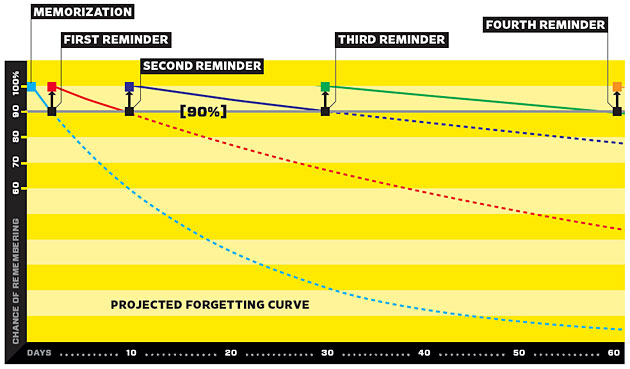
\includegraphics[width=11cm]{img/wired_forgetcurve.jpg}
\caption{Projected Forgetting Curves with Spaced Repetitions \cite{wolf_want_2008}}
\label{fig_projectedforgettingcurve}
\end{figure}

Figure \ref{fig_projectedforgettingcurve} shows an example of spaced repetition in
action. After initial memorisation, a student might revise the content when there
is a 90\% chance of recalling the content correctly -- which might be the following day.
After this first revision, the student is likely to remember the content for a longer
period of time and on day 10 will again have a 90\% chance of recall. This continues
for each subsquent revision, with each revision solidifying the content in the student's
mind and the chance of remembering diminishing at a slower rate over time.

As an added advantage, by prompting the user to recall and then to rate their answer -- the user
is in a sense being tested and thus actively engaging rather than passively `studying'.
Testing and the associated active retrieval has been shown to improve retention
significantly over passive study \cite{effects_of_recall_tests_1969},
\cite{retrieval_for_learning_2008}, \cite{power_of_testing_memory_2006}.

\begin{table}[h!]
\caption{Example of reviews for a single flash-card in spaced repetition}
\label{tbl_spacedrepetitionexample}
\begin{tabular}{|r|c|l|}
\hline
Review Date & Recall & New Interval \\
\hline
1 Jan & Incorrect & 0 days \\
1 Jan & Correct, difficult & 1 day \\
2 Jan & Correct, difficult & 2 days \\
4 Jan & Correct, easy & 5 days \\
9 Jan & Correct, easy & 12 days \\
21 Jan & Incorrect & 0 days \\
21 Jan & Correct, easy & 1 day \\
22 Jan & Correct, easy & 3 days \\
\ldots & \ldots & \ldots \\
\hline
\end{tabular}
\end{table}

Spaced repetition software automates this process by storing relevant data alongside each
flash-card in a database. The type of data stored depends upon the spaced repetition algorithm
used. Most algorithms store the current interval (in days) which represents the spacing, or
an estimate of how long a student should be able to remember the word between reviews.
On each successful review, the interval is increased and the card rescheduled based on
the interval. Of course this is not an exact science, sometimes the student will not be able to recall,
and some algorithms take this into account and adjust based on the difficulty of the
particular word. An example of how a card might be rescheduled
is shown in table \ref{tbl_spacedrepetitionexample}.

Unfortunately, little publicly available research on spaced repetition
algorithms has been carried out. Dempster (1988)
postulated several potential reasons that spaced repetition itself has failed 
to catch on in education, which include a lack of demonstration in school-like activities, the
relative recency of its development, and a lack of understanding of the effect
\cite{dempster_spacing_effect_1988}.
 
Nonetheless, spaced repetition is a valuable tool in this project because of its
inherent tracking of several parameters for each vocabulary item for each student.

\subsection*{SuperMemo 2 Algorithm (SM2)}
As one of the first spaced repetition applications available for personal computers,
SuperMemo and its algorithms paved the way for other applications such as Mnemosyne and
Anki (see section \ref{background_similarprojects}). Developed by Piotr
Wozniack\cite{wozniak_optimization_1990}, the \textit{SuperMemo 2} algorithm was an
enhancement over the \textit{SuperMemo} algorithm primarily in that it would differentiate 
between items based on their difficulty to memorise\cite{wozniak_optimization_1990}.

The SuperMemo algorithm reschedules flash-cards a number of days into the future, known
as the \textit{interval}, where the interval is defined as the function $I(n)$ with $n$ the
current repetition number. For the first repetition, the interval is simply one day.
For the second repetition, the interval increases to six days. 
\begin{equation}
I(1) := 1
\end{equation}

\begin{equation}
I(2) := 6
\end{equation}

For all $n \geq 3$, equation \ref{eqn_sm2_3} applies.

\begin{equation}
\label{eqn_sm2_3}
I(n) := I(n-1) \times EF
\end{equation}

$EF$ is defined as the \textit{easiness factor} of the flash-card. The easiness factor
of the flash-card is adjusted on each review based on the answer given by the user with
equation \ref{eqn_sm2_4}

\begin{equation}
\label{eqn_sm2_4}
EF := EF + (0.1 - (5 - q) \times (0.08 + (5 - q) \times 0.02))
\end{equation}

Where $q$ denotes the user's self-rated accuracy of recall, according to table \ref{tbl_sm2ratings}.
\begin{table}[h!]
\caption{User Rated Answers for the SuperMemo 2 Algorithm \cite{wozniak_optimization_1990}}
\label{tbl_sm2ratings}
\begin{tabular}{|c|l|}
\hline
5 & Perfect response \\
4 & Correct response after a hesitation \\
3 & Correct response recalled with serious difficulty \\
\hline
2 & Incorrect response; where the correct one seemed easy to recall \\
1 & Incorrect response; the correct one remembered \\
0 & Complete blackout. \\
\hline
\end{tabular}
\end{table}

The easiness factor is bounded by the values $1.1 \leq EF \leq 2.5$ where 1.1 indicates
the most difficult flash-cards and 2.5 indicates the easiest. Before a user begins studying a
flash-card for the very first time, the associated easiness factor is set to 2.5.

\section{Similar Projects} \label{background_similarprojects}
\subsection*{Memrise}
Memrise is a private company which produces web-based flashcard software. Memrise states
on their website: \textit{``Our memory experts have spent long, sleepless nights
tinkering with exotic algorithms so as to be able precisely to estimate the
point at which you're about to forget it.''} \cite{memrise_website}. Their implementation
details however have not been made public.

\subsection*{The Mnemosyne Project}
Mnemosyne is open source spaced repetition software collecting anonymised data from its many users in order
to evaluate the effectiveness of the implemented spaced repetition algorithm \cite{peter_bienstman_principles_2012}.
Mnemosyne uses a modified version of the Supermemo algorithm. Mnemosyne chose to avoid SuperMemo 3+ algorithms
due to their complexity, however has recently moved to the SuperMemo 11 algorithm \cite{peter_bienstman_principles_2012}.
The project does not appear to have produced any papers or research publications at this time.

\begin{figure}[h!]
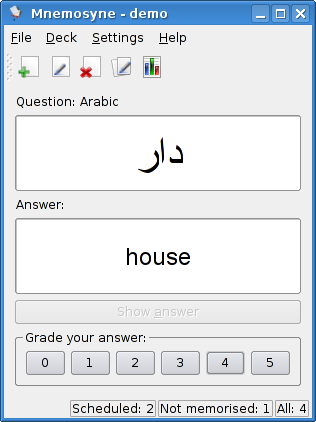
\includegraphics[width=4cm]{img/mnemosyne_screen.png}
\caption{Screenshot of Mnemosyne in use}
\end{figure}

\subsection*{Anki}
Anki is one of the most full-featured open-source spaced repetition applications available.
Anki allows users to attach images, sounds, and even embed \LaTeX \ equations in flash-cards. The
software is not designed for any research purposes but rather purely for learning and
review of information.

The developer of Anki decided against SuperMemo 3 and later algorithms instead opting for
the SuperMemo 2 algorithm because of the complexity that the SM3+ algorithms introduce \cite{anki_faq}.

\begin{figure}[h!]
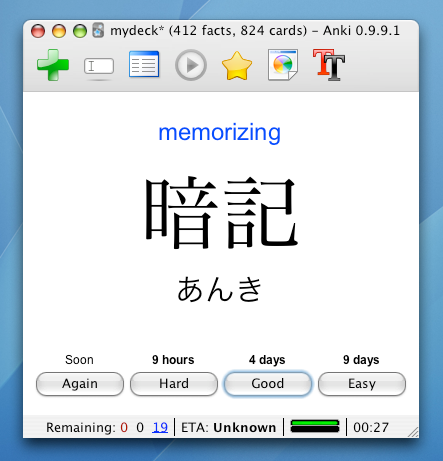
\includegraphics[width=6cm]{img/anki.png}
\caption{Screenshot of Anki in use}
\end{figure}